\documentclass[11pt,a4paper]{article}
\usepackage[margin=2.5cm]{geometry}
\usepackage{hyperref}
\usepackage{amsmath}
\usepackage{booktabs}
\usepackage{parskip}
\usepackage{listings}
\usepackage{xcolor}
\usepackage{microtype}
\usepackage{enumitem}
\usepackage{titling}
\usepackage[font=small,labelfont=bf]{caption}
\usepackage{graphicx} 
\hypersetup{
    colorlinks=true,
    linkcolor=black,
    urlcolor=blue,
    citecolor=black
}
\lstset{
    basicstyle=\small\ttfamily,
    backgroundcolor=\color{gray!10},
    frame=single,
    breaklines=true,
    columns=fullflexible
}
\title{\textbf{Project 2: Veterinarian Recommendation}\\[0.4em]
\large Data Analytics --- Spring 2026}
\author{Mehmet Fatih Tekin \and Vittoria Scocco}
% \date{19.04.2026}
\begin{document}
\setlength{\droptitle}{-2cm}
\maketitle
\noindent The full source code for this project is available on \href{https://github.com/Vitto28/Vet_Recc}{GitHub}.
 
% ─────────────────────────────────────────────────────────────────────────────
\section{Environment Setup}
\label{sec:setup}
% ─────────────────────────────────────────────────────────────────────────────
 
Place the dataset under a local directory of your choice. The notebook dynamic path resolution, the order of which is given on the \texttt{README.md} file. We recommend creating a file named \texttt{paths.local.json} in the project root with the path to the data, like so: \texttt{\{"data\_dir": "/absolute/path/to/your/data"\}}
 
% ─────────────────────────────────────────────────────────────────────────────
\section{Data Exploration}
\label{sec:exploration}
% ─────────────────────────────────────────────────────────────────────────────
 
Two are two datasets: one containing \textbf{ratings} (\texttt{ratings\_Pet\_supplies.csv}) with fields \texttt{user\_id}, \texttt{asin}, \texttt{rating}, and \texttt{timestamp}; and one containing product \textbf{metadata} (\texttt{meta\_Pet\_supplies.json}) with product attributes (title, brand, price, sales rank, categories, related items).
 
\subsection{Ratings dataset}
 
Table~\ref{tab:ratings_stats} summarises the key figures. As shown in Figure~\ref{fig:rating_dist}, the distribution is heavily skewed: roughly 60\,\% of all reviews are 5-star, producing a characteristic J-shape typical of voluntary online reviews. Both reviews-per-user and reviews-per-item follow power-law distributions, with most users having reviewed only one or two products. The resulting interaction matrix has a sparsity above 99.99\,\%, which can make collaborative filtering difficult.
 
\begin{table}[h]
\centering
\small
\begin{tabular}{@{}lr@{}}
\toprule
\textbf{Statistic} & \textbf{Value} \\
\midrule
Total reviews       & $\sim$1.2M \\
Unique users        & $\sim$740\,k \\
Unique items        & $\sim$145\,k \\
Mean rating         & 4.11 \\
Median rating       & 5.0 \\
Std deviation       & 1.39 \\
\% 5-star reviews   & $\sim$60\% \\
\% 1-star reviews   & $\sim$12\% \\
\bottomrule
\end{tabular}
\caption{Summary statistics for the ratings dataset.}
\label{tab:ratings_stats}
\end{table}
 
\begin{figure}[h]
  \centering
  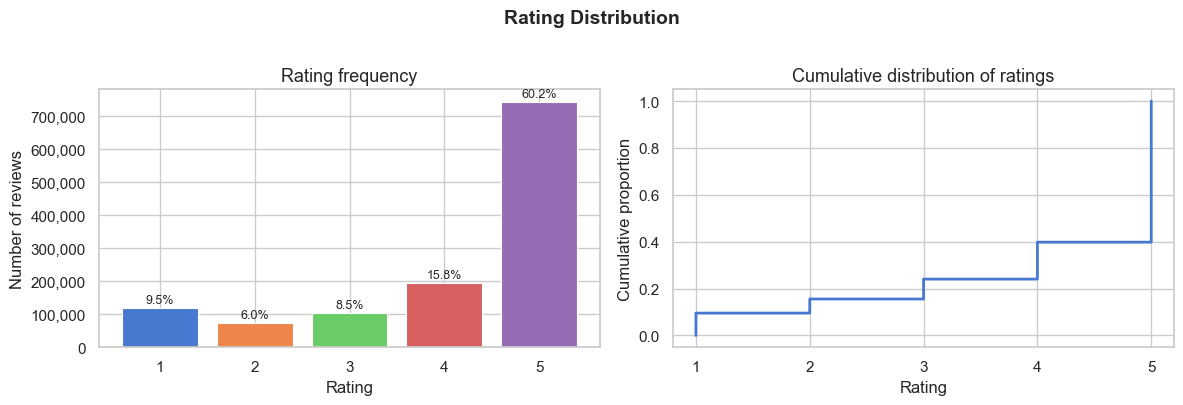
\includegraphics[width=0.85\linewidth]{figures/rating_distribution.png}
  \caption{Rating frequency (left) and cumulative distribution (right). About 60\,\% of reviews are 5-star.}
  \label{fig:rating_dist}
\end{figure}
 
\subsection{Metadata dataset}
 
The most notable quality issue is high missingness: over 50\,\% of products lack a brand and roughly 25\,\% have no price. Brand missingness spans many categories, but is higher for clothing, accessories, and carriers. Simulating a full drop of products with missing brand or price removes a large share of the catalogue and the ratings that reference it, so rather than straight up deleting these entries, it could be worth it to fill in these values with "defaults" (see Section~\ref{sec:preprocessing}).
 
Prices are highly right-skewed (median $\sim\$15$, mean $\sim\$30$), with a long tail of expensive items (kennels, aquarium equipment) that are not data errors. As shown in Figure~\ref{fig:price_rating}, there is no meaningful correlation between price and average rating ($r \approx 0$). Items with more reviews converge toward the overall mean (roughly .1), while low-review-count items show much higher variance. KONG is the most reviewed brand, followed by PetSafe and Midwest Homes for Pets; ratings for less popular brands are less reliable due to smaller sample sizes.
 
\begin{figure}[h]
  \centering
  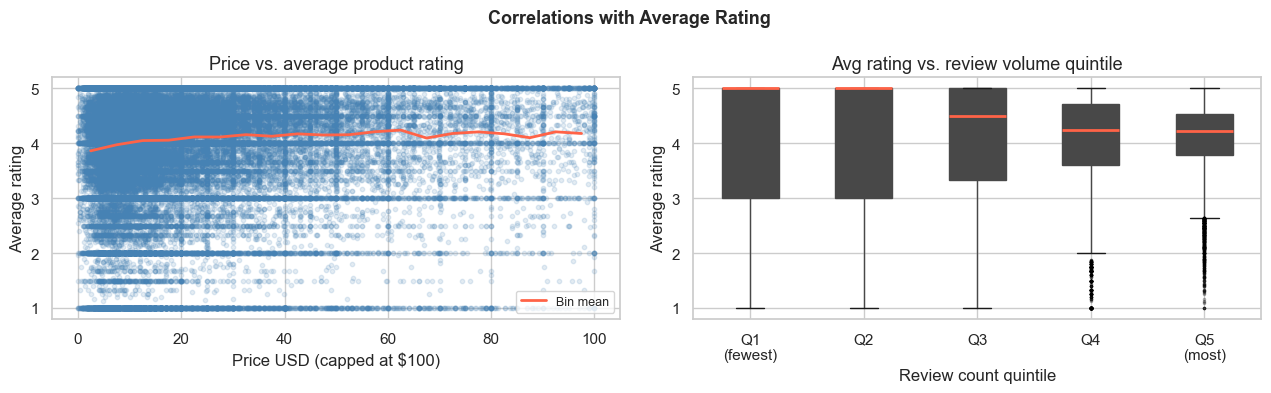
\includegraphics[width=0.85\linewidth]{figures/price_vs_rating.png}
  \caption{Price vs.\ average product rating (left) and average rating by review-count quintile (right). No meaningful price--rating correlation; high-review items converge to the mean.}
  \label{fig:price_rating}
\end{figure}
 
% ─────────────────────────────────────────────────────────────────────────────
\section{Pre-processing}
\label{sec:preprocessing}
% ─────────────────────────────────────────────────────────────────────────────
 
\textbf{Timestamps.} Unix timestamps are converted to \texttt{datetime}, with \texttt{year} and \texttt{month} columns extracted for time-aware splitting.
 
\textbf{Missing value handling.} Missing values are filled rather than dropped to preserve coverage. Brand \texttt{NaN}s are replaced with \texttt{"Unknown"}. Price and sales rank are filled with their respective global medians; binary missingness flags (\texttt{price\_was\_missing}, \texttt{rank\_was\_missing}) are retained so models can distinguish the engineered values from the observed values. Description and title gaps are filled with empty strings or \texttt{"Unknown"}; missing \texttt{related} entries become empty dicts.
 
\textbf{Log-transformation.} Both \texttt{price} and \texttt{sales\_rank} are log-transformed to reduce skewness and limit the influence of extreme values, producing more symmetric distributions better suited for modelling.
 
\textbf{Merging.} Ratings are aggregated per item (average rating, review count, std, date range) and left-joined to the cleaned metadata on \texttt{asin}, producing the item-level table used as input to the recommender pipeline.
 
 
% ─────────────────────────────────────────────────────────────────────────────
\section{Recommender system}
\label{sec:lsh}
% ─────────────────────────────────────────────────────────────────────────────
 
% ─────────────────────────────────────────────────────────────────────────────
\section{Results and Discussion}
\label{sec:results}
% ─────────────────────────────────────────────────────────────────────────────
 
 
\subsection{Summary?}
 
\section{Contributions}
 
% ─────────────────────────────────────────────────────────────────────────────
% REferences
% ─────────────────────────────────────────────────────────────────────────────
 
% \begin{thebibliography}{9}
 
% % \bibitem{pan2010}
% % Martin Potthast, Benno Stein, Alberto Barrón-Cedeño, and Paolo Rosso.
% % \textit{An Evaluation Framework for Plagiarism Detection}.
% % In \textit{Proceedings of the 23rd International Conference on Computational Linguistics (COLING 2010)}, pages 997-1005, 2010.
% % Dataset available at: \url{https://pan.webis.de/clef10/pan10-web/plagiarism-detection.html}
 
% % \bibitem{lsh_github}
% % MikaBattineni.
% % \textit{Plagiarism-Detection-LSH}.
% % GitHub repository, 2021.
% % \url{https://github.com/MikaBattineni/Plagiarism-Detection-LSH}
 
% \end{thebibliography}
 
\end{document}
